\chapter{Introduction}
\label{ch:introduction}

\section{Background}
\label{sec:background}

Rapid growth in the global building stock continues to drive energy demand. Residential buildings account for 70\% of total buildings energy demand, while commercial and public buildings comprise the remaining 30\% (IEA2025). Additionally, the buildings and construction sector accounted for 28 \% of global energy consumption, reinforcing its position as one of the world’s largest energy users in 2024. \parencite{unep2026} 

In the European Union, the building sector accounts for approximately 40\% of final energy consumption  and 36\% of its energy-related greenhouse gas emissions \parencite{epbd2024}. Reducing the energy demand and emissions of existing buildings is therefore central to European climate policy. Accordingly, the 2024 recast of the Energy Performance of Buildings Directive establishes the objective of achieving a zero-emission building stock by 2050 \parencite{epbd2024}. Reaching this objective requires reliable information on the existing building stock to support large-scale in energy performance assessment and the prioritisation of renovation measures \parencite{hettinga2023}.

The basic approach of UBEM is to apply physical models of heat and mass flows in and around buildings to predict operational energy use as well as indoor and outdoor environmental conditions for groups of buildings \parencite{reinhart2016}. UBEM requires the combination of several data sets as input, including climate data, building geometry, construction standards, and usage schedules. Figure~\ref{fig:ubem_workflow} illustrates a basic \ac{UBEM} workflow including input data, simulation, and output generation. Although such information can be collected in detail for individual buildings or small samples, doing so across larger urban areas is resource intensive and often impractical \parencite{reinhart2016}.

\begin{figure}[htbp]
	\centering
	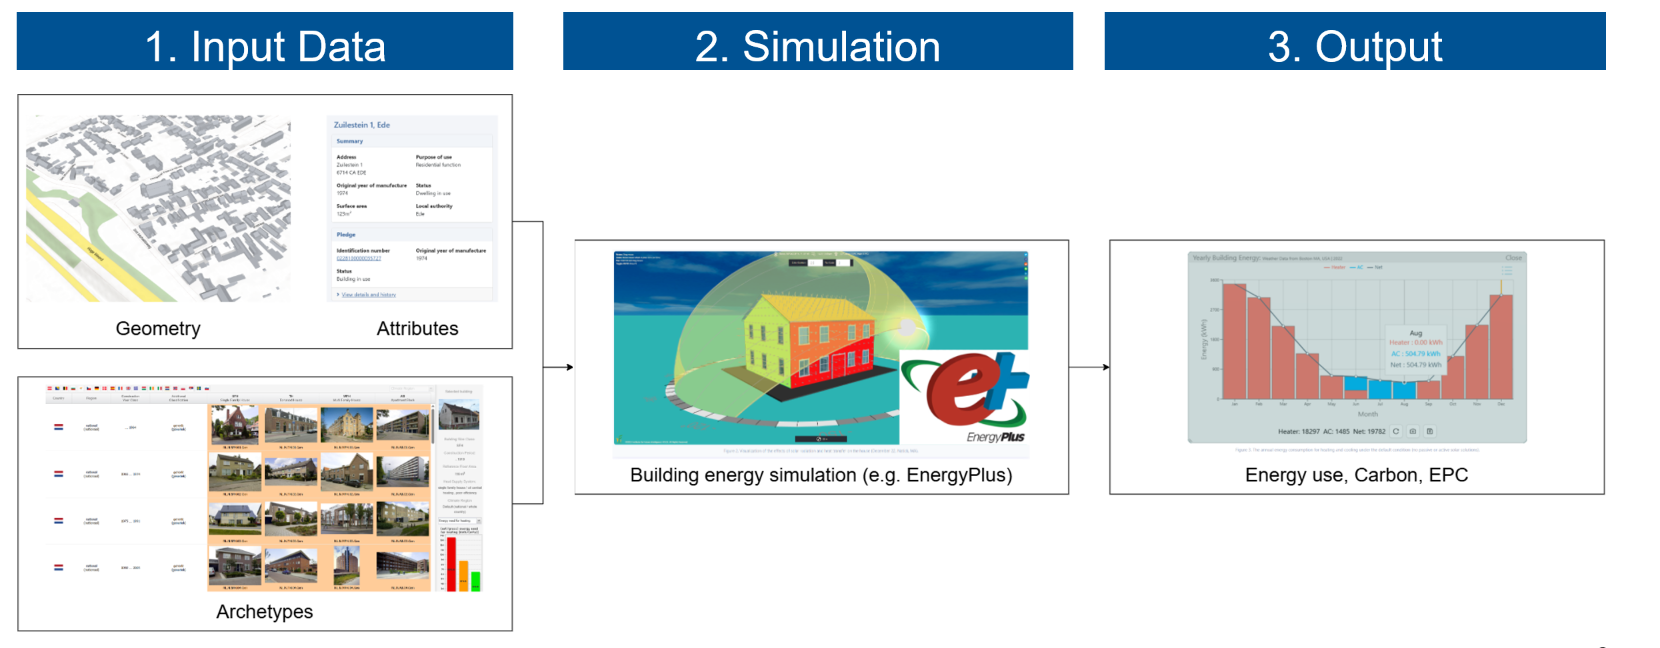
\includegraphics[width=\textwidth]{figures/fig/fig_3_1_UBEM_workflow}
	\caption{General workflow for urban building energy modelling. Geometry, semantic attributes, and archetype information provide inputs for simulation. The results support assessments of energy use, carbon emissions, and energy performance.}
	\label{fig:ubem_workflow}
\end{figure}

To address these data constraints, \ac{UBEM} workflows commonly use building archetypes to represent groups of buildings with similar physical and operational characteristics \parencite{reinhart2016,shen_archetype_2024}. The archetype approach has been extensively used in the context of national or regional bottom-up building stock models. Archetype generation consists of two complementary steps, segmentation and characterisation. Segmentation divides the building stock into groups according to building shape, age, use, climate, and technical systems. During characterisation, archetype buildings are defined using a complete set of thermal properties, including construction assemblies, usage patterns, and building systems \parencite{reinhart2016}. Depending on the scale of application and the segmentation parameters chosen, an archetype may represent from fewer than 50 to as many as 500,000 buildings \parencite{reinhart2016}.

In recent decades, typological approaches have been used to assess building energy performance at national, regional, and municipal scales across Europe \parencite{loga2016}. Among these approaches, the TABULA project provides archetype matrices for 20 European countries that classify residential buildings by construction period and size class \parencite{loga2016}. Figure~\ref{fig:tabula_example} shows the TABULA typology schema including national building stock models and exemplary buildings. Each archetype cell is associated with a set of representative as-built U-values for  building stock group rather than individual buildings. These national typologies provide a foundation for building stock models that estimate the energy consumption of the respective residential stocks \parencite{loga2016}.

\begin{figure}[htbp]
	\centering
	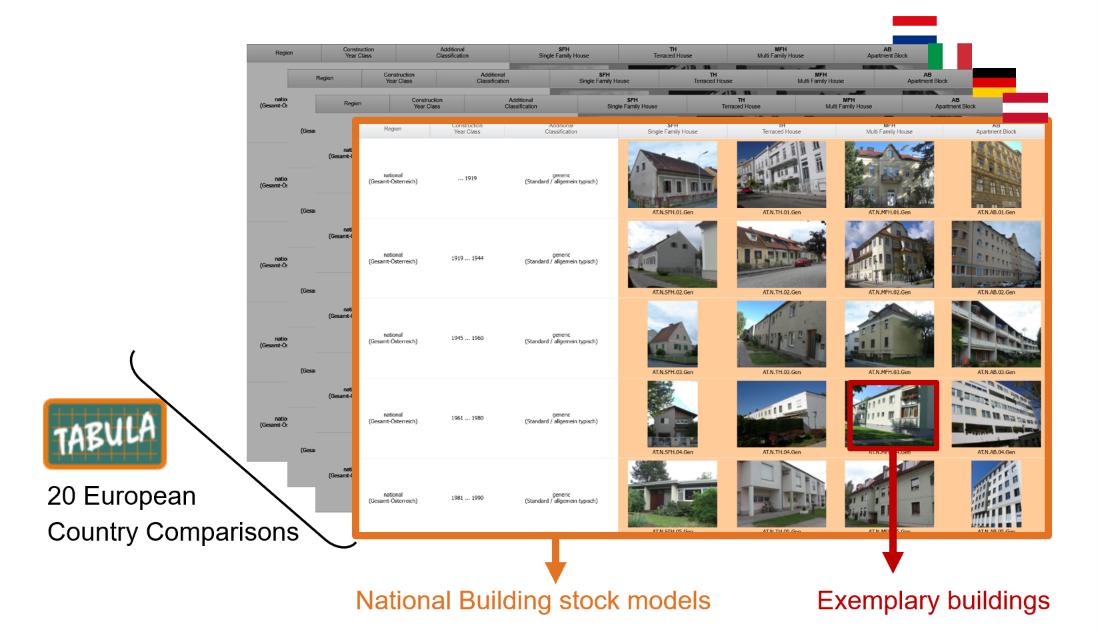
\includegraphics[width=\textwidth]{figures/fig/fig_1_1_tabula_example}
	\caption{TABULA typology concept. Structural information and residential building stock data from 20 European countries support the development of national building stock models and exemplary buildings \parencite{loga2016}.}
	\label{fig:tabula_example}
\end{figure}

\section{Motivation}
\label{sec:motivation}

The Netherlands provides a relevant setting for examining this information gap. Although its Energy Performance Certificate scheme was introduced in 2008, only approximately 3.8 million residential buildings had a valid registered certificate by the end of 2019, representing around 48\% of the residential building stock \parencite{caepbd2020}. Incomplete certificate and building-attribute coverage constrains consistent building-level assessment across the stock. Model-based estimates are not substitutes for formal certification, but they can support stock-level screening and preliminary renovation prioritisation where complete reference data are unavailable.

In archetype-based assessment, a practical bottleneck is the availability of building-level attributes needed for assignment and downstream analysis. This study focuses on building type, construction year, and floor count because they have distinct roles in the evaluated workflow. Building type and the construction period derived from construction year determine the TABULA-NL archetype cell, whereas floor count is retained as an additional predictor in downstream energy-class classification. TABULA-NL denotes the Dutch national typology within the European TABULA framework.

Remote sensing and \acf{SVI} offer scalable sources from which building characteristics can be inferred when structured attributes are incomplete. Prior research follows two broad routes. Attribute-mediated approaches infer building characteristics and subsequently use them in energy models or archetype assignment \parencite{garbasevschi2021,wurm2021,dabrock2025,liang2025}, whereas direct approaches predict energy-efficiency classes from street-view and aerial imagery \parencite{mayer2023uk,mayer2023dk}. These studies demonstrate that imagery and spatial data contain predictive information, but they do not establish how errors in inferred attributes affect later stages of an archetype-grounded workflow.

Among the studies reviewed here, none compares reference and \ac{SVI}-derived attributes for the same buildings while holding the data partitions and downstream classifier constant. Consequently, it remains unclear how the performance of different \ac{SVI} inference paradigms varies across attributes, how attribute errors propagate to TABULA-NL archetype assignment and associated thermal parameters, and how substituting inferred attributes affects downstream energy-class prediction and geographic transfer. The linked Dutch data provide a basis for examining these questions under a controlled and traceable protocol. These unresolved issues motivate the research objectives presented in the following section.

\section{Research Objectives}
\label{sec:research_objectives}

Large-scale applications of archetype-based \ac{UBEM} require metadata for assigning individual buildings to appropriate archetypes. This study focuses on three semantic attributes: building type, construction year, and floor count. When these attributes are incomplete or unavailable, \ac{SVI} may serve as an alternative source. The linked Dutch datasets provide administrative attributes, reconstructed geometry, and registered energy classes for the same buildings. This linkage enables a controlled comparison between \ac{SVI}-derived and reference attributes. In TABULA-NL, building type and construction period determine the archetype cell. This study derives construction period from construction year and retains floor count as an additional predictor in downstream energy class classification.

Accordingly, this study assesses the extent to which \ac{SVI}-derived attributes can substitute for reference attributes obtained from administrative records and reconstructed 3D building data in a TABULA-based building stock enrichment workflow. The assessment is limited to the evaluated population, tasks, and geographic setting. Specifically, this study addresses three research objectives:

\begin{enumerate}
	\item \textbf{Evaluate the predictive performance of \ac{SVI}-based extraction of building type, construction year, and floor count.}
	      Three inference paradigms are evaluated on the same attributes and data partitions: a fully fine-tuned \acf{CNN}, a frozen self-supervised backbone with supervised prediction heads, and \ac{VLM} inference without parameter updating.

	\item \textbf{Quantify agreement between \ac{SVI}-derived and reference TABULA-NL archetype assignments and the resulting differences in archetype-derived transmission heat transfer coefficients.}
	      Reference and \ac{SVI}-derived archetype assignments are compared using cell-level agreement metrics and differences in the resulting $H'_{tr}$ values.
	      Both calculations use the same reconstructed areas and window-to-wall ratio.
	      The resulting $H'_{tr}$ differences provide a physically weighted comparison of archetype assignments and do not constitute validation against measured heat loss.

	\item \textbf{Quantify the downstream performance change resulting from replacing reference attributes with \ac{SVI}-derived attributes, and evaluate transfer to Amsterdam as a held-out city.}
	      The controlled substitution analysis holds the evaluated buildings, data partitions, and downstream classifier constant while changing the attribute source.
	      The analysis also estimates the marginal contribution of individual attributes and evaluates transfer to Amsterdam after excluding the city from model development.
\end{enumerate}

To support these objectives, this study constructs a three-layer semi-synthetic building dataset grounded in TABULA. The provenance of every value is retained across the three layers. The reference layer combines administrative observations, reconstructed geometry, and EP-Online reference energy classes. The vision-inference layer stores \ac{SVI}-derived attributes. The synthetic archetype layer records the TABULA cells and parameters assigned deterministically from reference or inferred attributes. Using this layered structure, this study evaluates how substituting \ac{SVI}-derived attributes for reference attributes affects performance in downstream energy class classification.
